%% Esqueleto base de la presentacion
%%% No agregar las paginas con un include
%%% Lo que quieran aportar deben ser usuarios del TRAC

\documentclass{beamer}
\usepackage[english,activeacute]{babel}
\usepackage[utf8]{inputenc}
\usepackage{listings}
\usepackage{algorithmic}
\usepackage{color}

\definecolor{gray2}{rgb}{100,100,100}
\definecolor{red}{rgb}{255,0,0}
\definecolor{blue}{rgb}{0,0,255}
\definecolor{gray97}{gray}{.97}
\definecolor{gray75}{gray}{.75}
\definecolor{gray45}{gray}{.45}

\newcommand{\blue}{\textcolor{blue}}
\newcommand{\red}{\textcolor{red}}
\newcommand{\green}{\textcolor{green}}


\usetheme[pageofpages=of,% String used between the current page and the
                         % total page count.
          alternativetitlepage=true,% Use the fancy title page.
          titlepagelogo=img/logo,% Logo for the first page.
          watermark=,% Watermark used in every page.
          watermarkheight=100px,% Height of the watermark.
          watermarkheightmult=4,% The watermark image is 4 times bigger
                                % than watermarkheight.
          ]{Torino}

\usecolortheme{nouvelle}


\lstset{ frame=Ltb,
     framerule=0pt,
     aboveskip=0.5cm,
     framextopmargin=3pt,
     framexbottommargin=3pt,
     framexleftmargin=0.4cm,
     framesep=0pt,
     rulesep=.4pt,
     backgroundcolor=\color{gray97},
     rulesepcolor=\color{black},
     %
     stringstyle=\ttfamily,
     showstringspaces = false,
     basicstyle=\tiny\ttfamily,
     %commentstyle=\color{gray45},
     %keywordstyle=\bfseries,
     %
     numbers=left,
     numbersep=13pt,
     numberstyle=\tiny,
     numberfirstline = false,
     breaklines=true,
	 emph = {[1]\_\_device\_\_,\_\_global\_\_,\_\_syncthreads,pthread\_create,pthread\_join,pragma,omp,parallel,private, threadIdx, blockDim, blockIdx,cudaThreadSynchronize},
	 emphstyle={[1]\color{blue}},
   }

% minimizar fragmentado de listados
\lstnewenvironment{listing}[1][]
   {\lstset{#1}\pagebreak[0]}{\pagebreak[0]}

\lstdefinestyle{consola}
   {basicstyle=\scriptsize\bf\ttfamily,
    backgroundcolor=\color{gray75},
   }
\lstdefinestyle{C}
   {language=C,
   }

\author[C. Maureira]{\large Cristián Maureira Fredes\\\normalsize \textcolor{gray}{cmaureir@csrg.cl}}
\title[n-body benchmark]{A n-body particle-particle algorithm benchmark}
\subtitle{Using many and multi cores approaches.}
\institute[UTFSM]{Departamento de Informática\\Universidad Técnica Federico Santa María}
\date{\today}

\begin{document}
\begin{frame}[t,plain]
\titlepage
\end{frame}
% Introduccion a n-body.\\
The $n-body$ problem is widely used in different investigation
related to the formation and evolution of several other problems,
as well as planetary clusters, star clusters, galaxy clustering, back holes,
universe large structure formation, among others.

The main idea of the $n-body$ problem is to simulate the
motion of a certain particle number, interacting gravitationally
between each other by a force caused by other bodies.
So, looking the motion of stars and planets, the gravity
is the main character of this phenomena.
This movement is defined by some differential equations
proposed in first instance by Newton.

%Definición del problema.
The \emph{n-body} problem is the problem of
predict the movement of a particles set of celestial objects,
which interact with each other due to the gravitational force.

Each celestial object will have a determinate \emph{mass} $(m)$
and a specific location in 3D space
$(x, y, z)$, in addition to an initial velocity
determined in each direction $(v_{x}, v_{y}, v_{z})$ and finally
will have some initial zero acceleration $(a_{x}, a_{y}, a_{z})$.
It should be noted that the \emph{position}, the \emph{velocity} and \emph{acceleration}
will be updated depending on the interaction with other bodies
which follow the gravitational force formula,
which is defined by:

\begin{eqnarray}
    f_{ij} =G \cdot \frac{m_i \cdot m_j}{||r_{ij}||^{2}} \cdot \frac{r_{ij}}{||r_ij||}
\end{eqnarray}

where the initial position are $x_{i}$,
the velocities are $v_{i}$,
having an $i$, between values, $1\leq i\leq N$,
the $i$ and $j$ bodies mass is determined by $m_{i}$ and $m_{j}$
where $r_{ij} = (x_{j} - x_{i})$ is the distance vector between the $i$ and $j$ bodies
and then $G$, gravitational constant. ($6.67428\times 10^{-11} m^{3} kg^{-1} s^{-2}$)

A classic example of what is the \emph{n-body} problem
is the planets movement in our solar system,
which is affected by the Sun properties
and as all the other bodies that are between their orbits.

The interest factor of the \emph{n-body} problem
is that numerical algorithms are developed to solve
the dynamics of this problem can be applied not only in the astrophysics area,
with fields such as \emph{Celestial mechanics}, \emph{Dense stellar systems},
\emph{Sphere of Influence of a massive BH}, and \emph{Galaxy dynamics and cosmology},
but it also widely used in the fluid dynamics field,
which for example may be reflected in the work of Gingold et al.~\cite{Gingold}
which takes as its main objective a method of resolution of physical models,
more than the same particle interaction.

Another important area in fluid dynamics are the \emph{Vortex Methods},
which are a technique for various turbulent flows simulation of a particular fluid.
However, applications are not only in theory, for example,
have been made smoke simulations in real time for video games development use~\cite{Gourlay}.

% 	¿Por qué es dificil?
% 		¿Es NP-completo?
% 		Debilidades de lo existente
% 		Costo versus calidad de las soluciones

Solving the \emph{n-body} problem consists of three
key issues that will be determinate the calculation difficulty.

First, for this problem is required an initial scenario
so there are alternatives, which can be
randomly generated positions, which itself carries a problem,
or take existing models to generate a baseline,
as \emph{Plummer model} although unrealistic,
attempts to deliver a distributed bodies scenario
based on the density of a certain system.

Another important aspect is that as we work with the bodies interaction,
we need to use a method to integrate the motion equations,
in order to update \emph{position}, \emph{speed}
and \emph{acceleration}.

This is where various methods widely known have been used,
such as \emph{Forward and Backward Euler} which are not recommended
due to low precision. From that point that other methods have improved
the operation of the motion equations, such as \emph{Leapfrog integration}.
Finally, the recommended methods are \emph{Runge Kutta} and \emph{Two-stepAdams Bashworth}
which have a much better accuracy than previous methods, but are
highest level of calculation.

Finally, the most important point to this problem is the force calculation between the particles,
being the main focus of the present work, because if we consider the exerted force on a particle
is determined by all other particles in a given system, the order of the algorithm grows
quadratically by increasing the amount of particles, matter by which various researchers have
conducted techniques to reduce the order of $O(n^2)$ it holds in its initial version,
taking an approach called \emph{Particle-Particle}.

%Hablar de las características del problema: (explicar 2 o mas metodos)
%-Poblacion inicial.
%-Metodo de integracion.
%-Metodo calculo fuerza.

%Estado del Arte

% Criticar soluciones existentes, no agresivamente.
% 	Analisis -> Criterio (que usaremos para analizar nuestro propio trabajo)
% 	Definir criterios de evaluación.
% 	Explicar lo que implica y por que son importantes.

% Introduccion del estado del arte explicando enfoque

% formula de calculo de fuerza

% Explicación de métodos para calculo fuerza


\begin{frame}[fragile]
	\frametitle{Algorithm}
	\framesubtitle{Pseudocode}
	\begin{center}
		\begin{algorithmic}
			\STATE $updateAccelerations()$
			\FOR {$counter = 0 \to iterations$}
			    \STATE $updatePositions()$
			    \STATE $updateAccelerations()$
			    \STATE $updateVelocities()$
			\ENDFOR
		\end{algorithmic}
	\end{center}
\end{frame}

\begin{frame}[fragile]
    \frametitle{Algorithm}
    \framesubtitle{Profiling}
     \begin{itemize}
         \item Using \texttt{gprof}.
     \end{itemize}
     \begin{table}[h!t]
        \centering
        \scriptsize
        \begin{tabular}{|c|c|c|c|c|}
           \hline
           {\bf \% Time } & {\bf self seconds} & {\bf calls} & {\bf total ms/call} & {\bf name} \\\hline
             99.74   &  51.20   &  1002   &  51.10  & updateAccelerations() \\\hline
              0.08   &   0.04   &  1001   &   0.04  & updateVelocities()\\\hline
              0.02   &   0.01   &  1001   &   0.01  & updatePositions()\\\hline
              0.00   &   0.00   &     1   &   0.00  & checkAndInit(int, char const**)\\\hline
        \end{tabular}
        \caption{Serial implementation, using 1024 bodies}
     \end{table}
\end{frame}


\begin{frame}[fragile]
\frametitle{Algorithm}
\framesubtitle{OpenMP}
\begin{lstlisting}[style=C]
void updateAccelerations(){
    int i,j;
    for (i = 0; i < n; i++) {
        bodies[i].ax = bodies[i].ay = bodies[i].az = 0;
    }
    #pragma omp parallel for private(j)
    for (i = 0; i < n; i++) {
        for(j=0; j<n; j++){
            if(j != i)
                accelerationCalc(i,j);
        }
    }
}
\end{lstlisting}
\end{frame}

\begin{frame}[fragile]
\frametitle{Algorithm}
\framesubtitle{Pthreads}
\begin{lstlisting}[style=C]
void updateAccelerations(){
    int i;

    for (i = 0; i < n; i++) {
        bodies[i].ax = bodies[i].ay = bodies[i].az = 0;
    }
    int bound = n/cores;
    for (i = 0; i < cores; i++) {
        threads[i].ini = i * bound;
        threads[i].end = threads[i].ini + bound;
        pthread_create(&threads[i].thread, NULL , accelerationCalc, (void *)&threads[i]);
    }

    for(int j=0 ; j < cores ; ++j){
        pthread_join(threads[j].thread, NULL);
    }

}
\end{lstlisting}
\end{frame}

\begin{frame}[fragile]
\frametitle{Algorithm}
\framesubtitle{CUDA}
\begin{lstlisting}[style=C]
__device__ void update_accelerations(particle *d_bodies,int n){

    int i = threadIdx.x + blockDim.x * blockIdx.x;
    int j;

    if (i < n){
        for(j=0; j<n; j++){
            if(j != i)
                accelerationCalc(i,j);
        }
    }
}
\end{lstlisting}
\end{frame}


\begin{frame}[fragile]
\frametitle{Algorithm}
\framesubtitle{CUDA}

\begin{lstlisting}[style=C]
  nbody<<< blockNum, threadsPerBlock >>> (d_bodies,ite,dt,n);
  cudaThreadSynchronize();
\end{lstlisting}

\begin{lstlisting}[style=C]
__global__ void nbody(particle *d_bodies,float ite, float dt, int n){

    float t;
    reset_accelerations(d_bodies,n);
    __syncthreads();
    update_accelerations(d_bodies, n);
    __syncthreads();

    for (t = 0.0; t < ite; t += dt){
        update_positions(d_bodies,dt,n);
        __syncthreads();
        reset_accelerations(d_bodies,n);
        __syncthreads();
        update_accelerations(d_bodies,n);
        __syncthreads();
        update_velocities(d_bodies,dt,n);
        __syncthreads();
    }
}
\end{lstlisting}
\end{frame}

\frame
{
\frametitle{Results}
\framesubtitle{Hardware and Software configuration}
\begin{itemize}
    \item CPU: 16 x Intel(R) Xeon(R) CPU E5520  @ 2.27GHz
    \item RAM: 12 GB
    \item Graphic Card: 2 x nVidia Tesla C1060.
    \begin{itemize}
        \item 1 GPU with 240 cores @ 1.3 GHz
        \item Memory: 4GB
    \end{itemize}
    \item OS: Scientific Linux SL release 5.6 (Boron)
    \item Kernel: 2.6.18-238.12.1.el5 x86\_64 GNU/Linux
\end{itemize}
}


\frame
{
\frametitle{Results}
\framesubtitle{OpenMP}
\begin{center}
    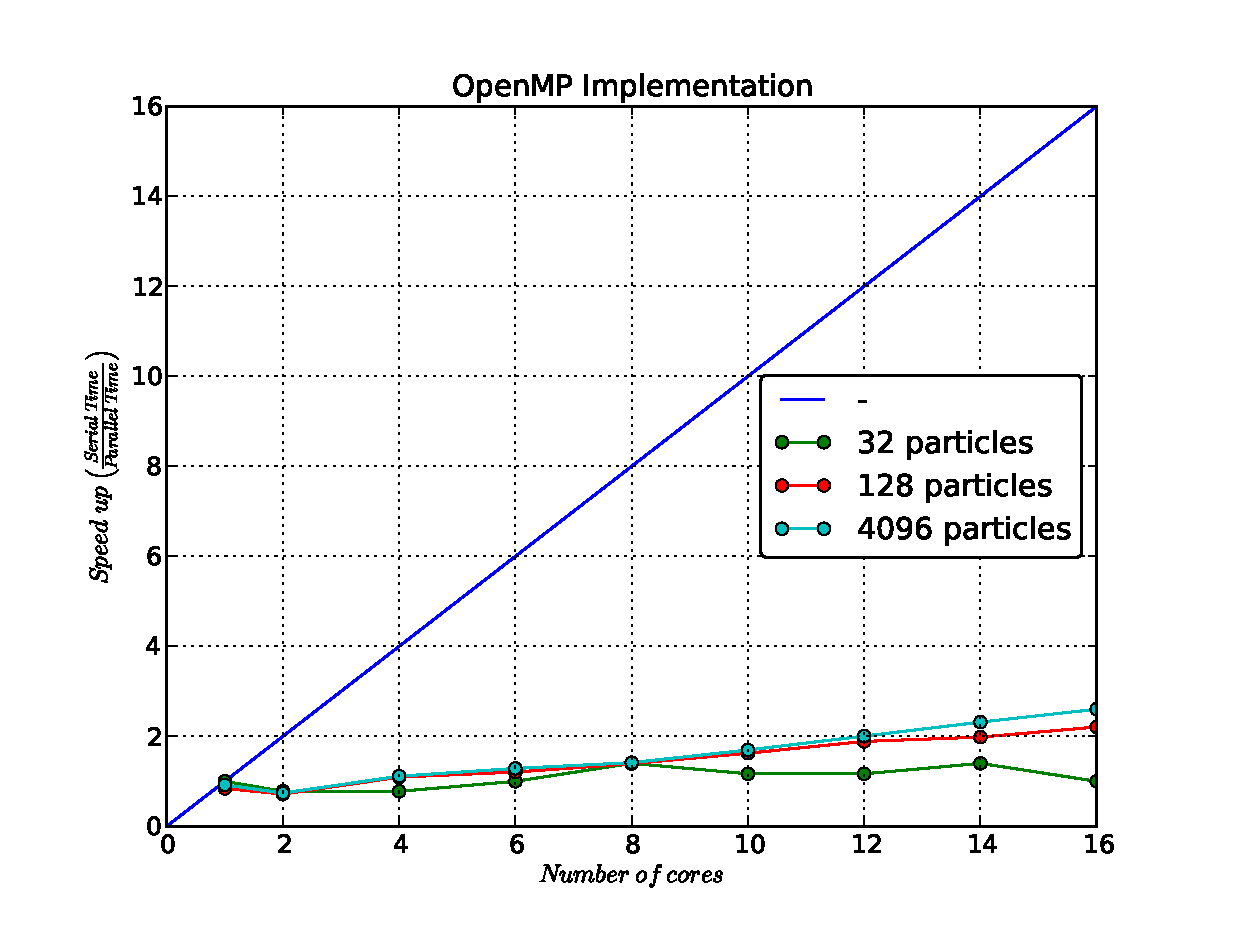
\includegraphics[width=0.8\textwidth]{img/openmp}
\end{center}
}

\frame
{
\frametitle{Results}
\framesubtitle{Pthreads}
\begin{center}
    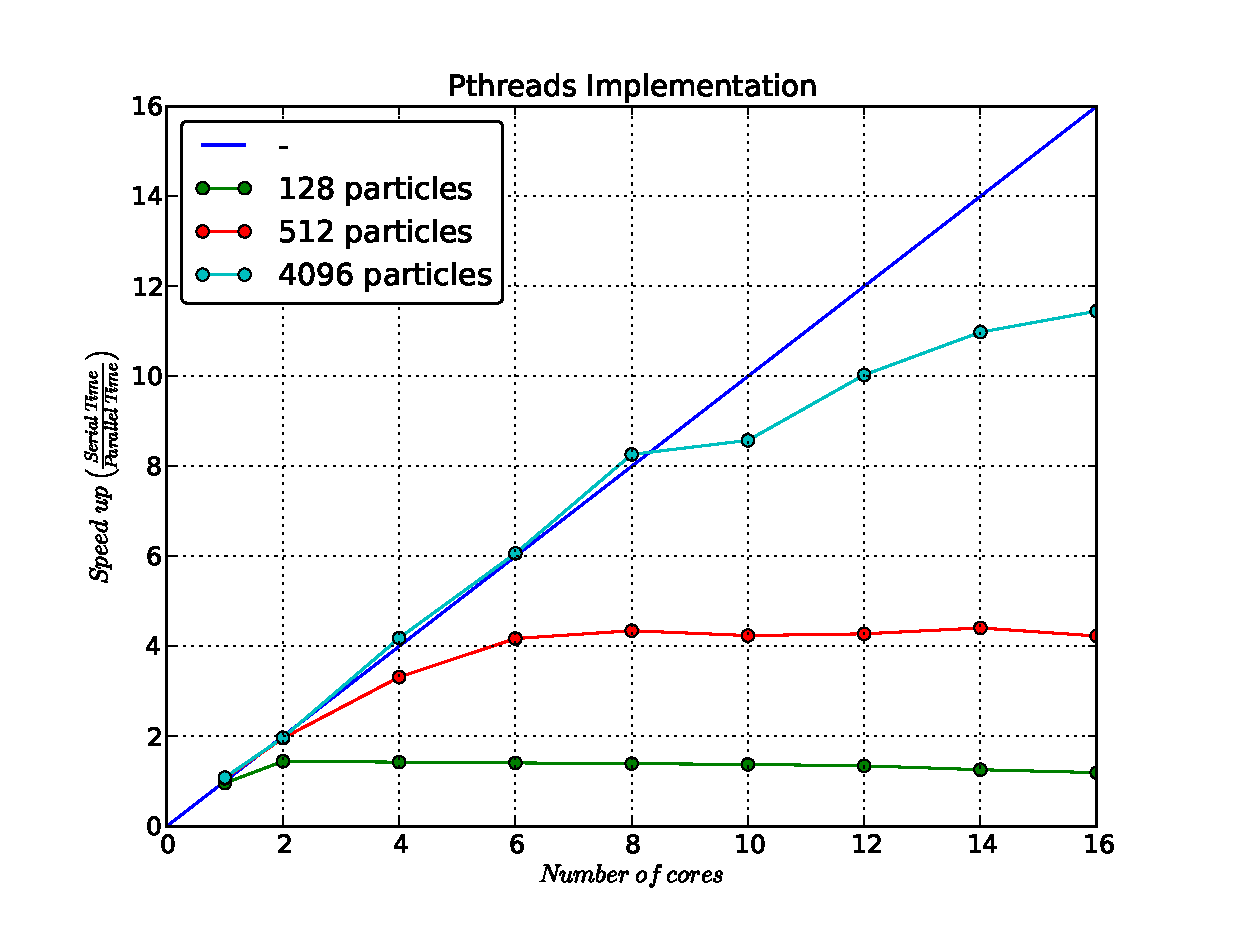
\includegraphics[width=0.8\textwidth]{img/pthreads}
\end{center}
}

\frame
{
\frametitle{Results}
\framesubtitle{CUDA}
\begin{center}
    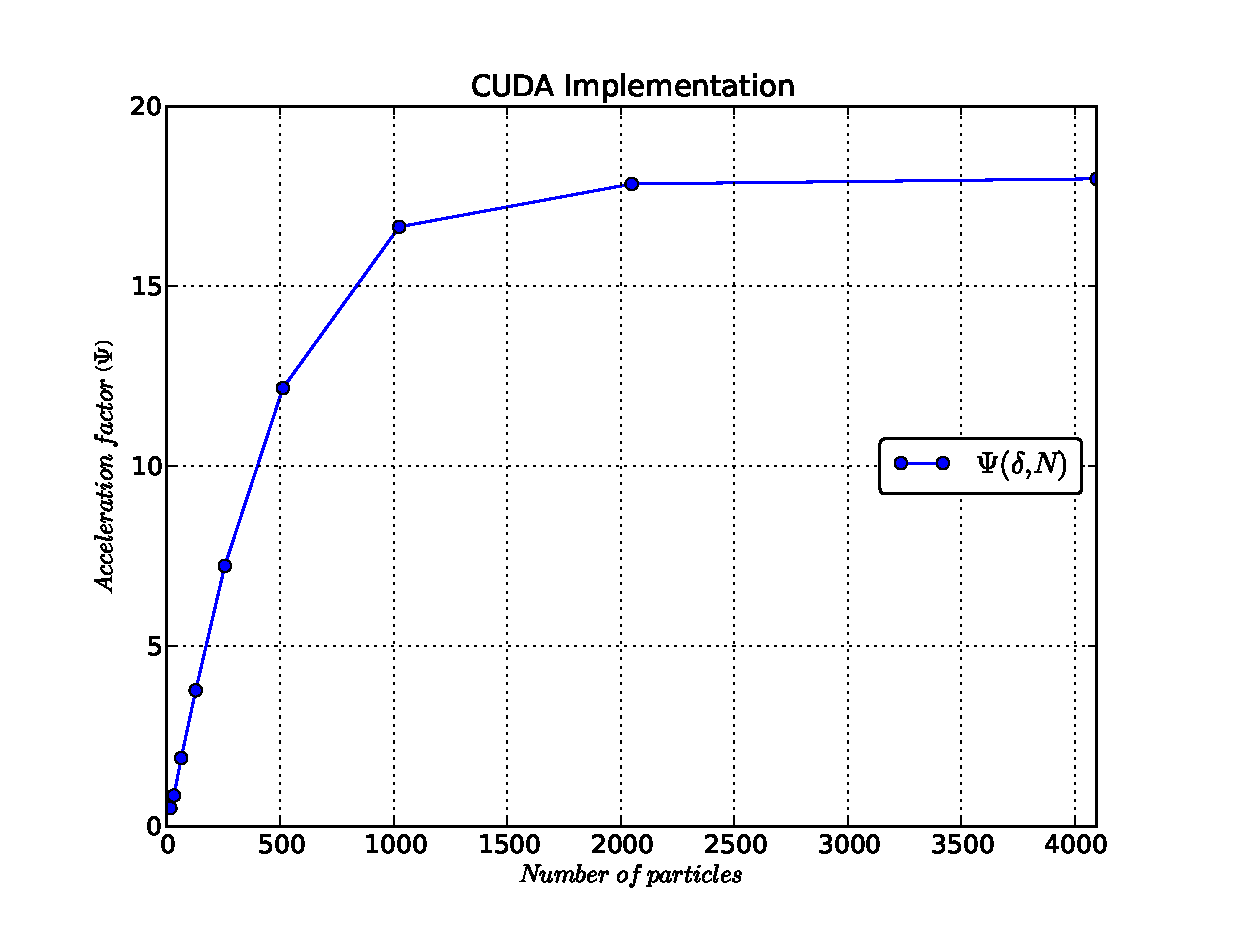
\includegraphics[width=0.8\textwidth]{img/cuda}
\end{center}
}

\frame
{
\frametitle{Results}
\framesubtitle{General}
\begin{center}
    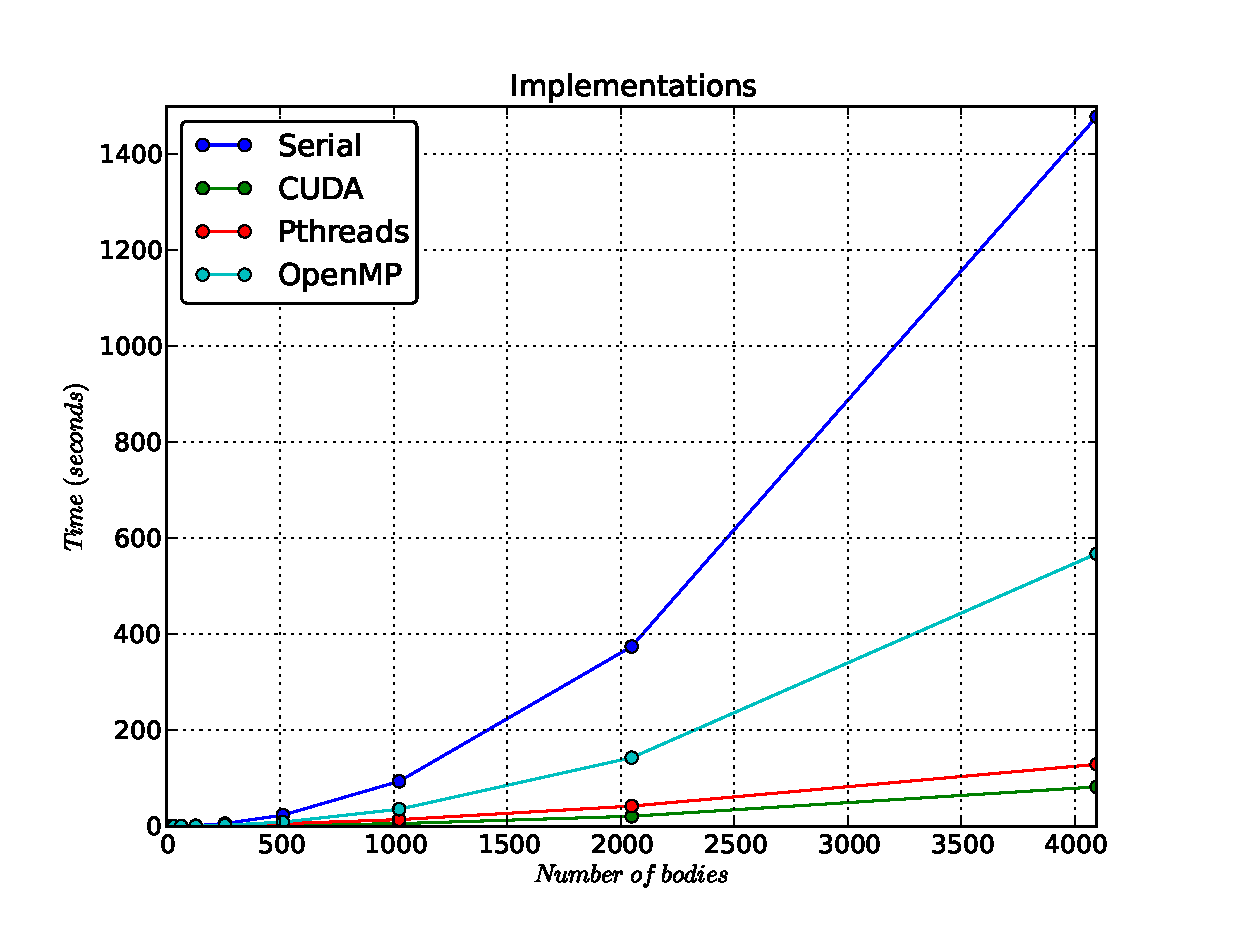
\includegraphics[width=0.8\textwidth]{img/all}
\end{center}
}

\frame
{
\frametitle{Results}
\framesubtitle{Acceleration}
\begin{center}
    \begin{tabular}{|c|c|}
        \hline
        \textbf{Implementation} & \textbf{Velocity} \\\hline
        Serial  & 1x  \\\hline
        OpenMP  & 3x  \\\hline
        Pthread & 11x \\\hline
        CUDA    & 18x \\\hline
    \end{tabular}
\end{center}
}

\begin{frame}[t,plain]
\titlepage
\end{frame}
\end{document}
